\parindent=0em
\subsection{Tecnologías en realidad aumentada}
\noindent


En primer lugar, un sistema básico de realidad aumentada~\cite{arhardwarerequirements} está formado al menos por tres tipos de elementos: sensores, procesadores y \textit{displays}. Los sensores son los encargados de obtener información del entorno y transmitírsela a la aplicación, los procesadores gestionan dicha información y los \textit{displays} son los dispositivos en los que se muestra la información de la aplicación.\\

Existen distintos tipos de sensores como los que aportan información sobre el nivel de luz del ambiente o la temperatura, aun así, los sensores más importantes son los que generan información sobre posición y orientación para conocer la pose y ubicación del usuario, este seguimiento del usuario se conoce como \textit{tracking}.\\

Se pueden distinguir distintos tipos de \textit{tracking} en función de los componentes que se utilicen para generar la información referente al usuario. Esta búsqueda de la pose del usuario se puede dividir~\cite{tracking1} en las siguientes técnicas:  

\begin{itemize}
    \item \textbf{Técnicas basadas en sensores:} Se utilizan sensores magnéticos, acústicos, inerciales o mecánicos entre otros. Por ejemplo, el \textit{tracking} con sensores mecánicos se realiza atando enlaces al objeto el cual se quiere realizar este seguimiento. Los enlaces tienen sensores que aportan información sobre el ángulo que se forma entre la unión de varios enlaces.\\
    
    %potenciometro https://www.iberobotics.com/producto/potenciometro-lineal-b10k-10k/
    
    Normalmente se utiliza un potenciómetro (figura \ref{fig:potenciometro}) en las uniones para obtener el voltaje, de este modo, cuando el ángulo entre los enlaces cambia, varía la resistencia del potenciómetro haciendo que cambie el valor del voltaje. Gracias a este componente se puede conocer la posición y orientación del objeto.
    
    \begin{figure}[H]
    \centering
    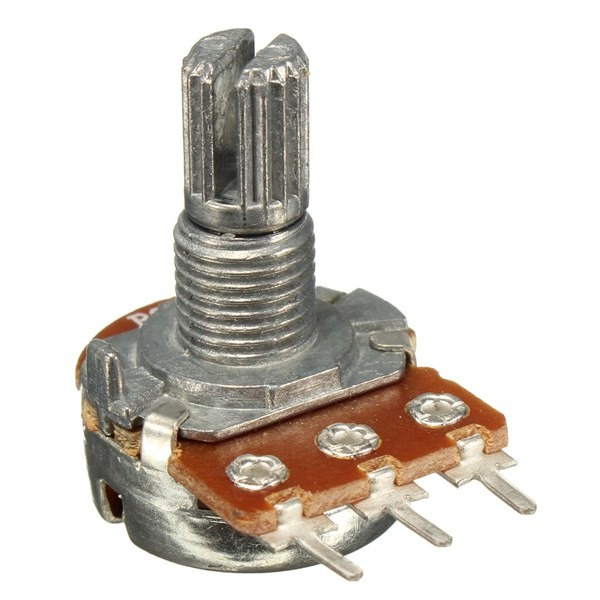
\includegraphics[scale=0.14]{Images/Estado del arte/potenciometro.jpg}
    \caption{Potenciómetro.}
    \label{fig:potenciometro}
\end{figure}

    Por otra parte, el seguimiento mediante sensores magnéticos~\cite{magneticIntro} es otra de las opciones del \textit{tracking} con sensores. El \textit{tracking} magnético se basa en la generación de un campo magnético de un transmisor para medir dicho campo en un receptor colocado en el objeto al cual se quiere hacer el seguimiento~\cite{magneticExplanation}. De esta forma se calcula la posición del objeto en relación al transmisor.\\
    
    Los campos magnéticos generados por el emisor pueden ser distorsionados por cualquier elemento metálico cercano, es por ello que este proceso no es una forma de seguimiento fiable por si sola para calcular la pose del objeto de forma exacta, ya que genera error en su estimación.\\
    

    \item \textbf{Técnicas basadas en la visión:} Estas son las técnicas más comunes, en ellas, se utiliza la visión por computador para obtener la información sobre el usuario. La visión por computador o visión artificial~\cite{visionporcomputador} es la transformación de datos de una cámara a una nueva representación, además, es necesario que estos datos incluyan información sobre la posición de la cámara (si se encuentra encima de un vehículo, por ejemplo).\\
    
    Dicha visión por computador se basa en encontrar una correspondencia entre puntos característicos de la imagen 2D y el entorno en 3D. De esta forma, la pose del elemento del cual se quiere hacer el seguimiento, se puede obtener proyectando las coordenadas 3D de los puntos característicos sobre las coordenadas de la imagen 2D y minimizando la distancia hacia estos.
    
    \item \textbf{Técnicas híbridas:} Las técnicas híbridas surgen de la necesidad de una precisión mayor en algunas aplicaciones debido a la robustez de las mediciones que se obtienen al hacer \textit{tracking} mediante sensores o por visión. Se llegó a la conclusión de que se podían combinar las técnicas por sensores con las técnicas que utilizan visión por computador, de esta manera, se saca partido a la velocidad de los sensores frente a la visión por computador y se complementa la robustez de los sensores con la precisión de las técnicas por visión. 
    
    Estas combinaciones permiten afinar el \textit{tracking}, por ejemplo, en una aplicación en el exterior en entornos como ciudades~\cite{hybridtrackingUrban} donde el nivel de distorsión es elevado y los sensores utilizados tradicionalmente (GPS y brújula magnética) son imprecisos.
    
    Para finalizar, un ejemplo de modelo híbrido es el modelo que combina información obtenida por el giroscopio y visión por computador basada en líneas~\cite{robustHybridmodel}, en él, se hace uso del giroscopio para predecir la orientación y la posición de las líneas de las imágenes que luego corrige la visión por computador.
    
\end{itemize}

Otra técnica comunmente utilizada en realidad aumentada es la tecnología SLAM~\cite{arSLAM} (del inglés Simultaneous Localization and Mapping) la cual consiste en una serie de algoritmos utilizados para calcular la posición del objeto del cual se hace el seguimiento, además, realiza una reconstrucción 3D del entorno. En el caso de estar utilizando un dispositivo móvil a la hora de aplicar SLAM se utiliza la información de la cámara, acelerómetro y giroscopio, también, puede complementarse esa información con la obtenida del GPS, sensores de luz o incluso cámaras de profundidad.